% Judul dokumen
\title{Buku Tugas Akhir ITS}
\author{Priyanto, Helmika Mahendra}

\newcommand\myName{HELMIKA MAHENDRA PRIYANTO}

% Pengaturan ukuran teks dan bentuk halaman dua sisi
\documentclass[10pt,twoside]{report}

% Pengaturan ukuran halaman dan margin
\usepackage[a5paper,top=25mm,left=25mm,right=20mm,bottom=25mm]{geometry}

% Pengaturan ukuran spasi
\usepackage[singlespacing]{setspace}

% Pengaturan format bahasa
\usepackage[indonesian]{babel}

% Pengaturan detail pada file PDF
\usepackage[pdfauthor={\@author},bookmarksnumbered,pdfborder={0 0 0}]{hyperref}

% Pengaturan jenis karakter
\usepackage[utf8]{inputenc}

% Pengaturan pewarnaan
\usepackage[table,xcdraw]{xcolor}

% Pengaturan kutipan artikel
\usepackage[numbers]{natbib}

% Package lainnya
\usepackage{changepage}
\usepackage{enumitem}
\usepackage{eso-pic}
\usepackage{etoolbox}
\usepackage{graphicx}
\usepackage{lipsum}
\usepackage{lmodern}
\usepackage{longtable}
\usepackage{tabularx}
\usepackage{wrapfig}

% Definisi untuk "Hati ini sengaja dikosongkan"
\patchcmd{\cleardoublepage}{\hbox{}}{
  \thispagestyle{empty}
  \vspace*{\fill}
  \begin{center}\textit{[Halaman ini sengaja dikosongkan]}\end{center}
  \vfill}{}{}

% Pengaturan penomoran halaman
\usepackage{fancyhdr}
\fancyhf{}
\renewcommand{\headrulewidth}{0pt}
\pagestyle{fancy}
\fancyfoot[CE,CO]{\thepage}
\patchcmd{\chapter}{plain}{fancy}{}{}
\patchcmd{\chapter}{empty}{plain}{}{}

% Pengaturan format judul bab
\usepackage{titlesec}
\titleformat{\chapter}[display]{\bfseries\Large}{BAB \centering\Roman{chapter}}{0ex}{\vspace{0ex}\centering}
\titleformat{\section}{\bfseries\large}{\MakeUppercase{\thesection}}{1ex}{\vspace{1ex}}
\titleformat{\subsection}{\bfseries\large}{\MakeUppercase{\thesubsection}}{1ex}{}
\titleformat{\subsubsection}{\bfseries\large}{\MakeUppercase{\thesubsubsection}}{1ex}{}
\titlespacing{\chapter}{0ex}{0ex}{4ex}
\titlespacing{\section}{0ex}{1ex}{0ex}
\titlespacing{\subsection}{0ex}{0.5ex}{0ex}
\titlespacing{\subsubsection}{0ex}{0.5ex}{0ex}

% Pengaturan format potongan kode
\usepackage{listings}
\definecolor{comment}{RGB}{0,128,0}
\definecolor{string}{RGB}{255,0,0}
\definecolor{keyword}{RGB}{0,0,255}
\lstdefinestyle{codestyle}{
  commentstyle=\color{comment},
  stringstyle=\color{string},
  keywordstyle=\color{keyword},
  basicstyle=\footnotesize\ttfamily,
  numbers=left,
  numberstyle=\tiny,
  numbersep=5pt,
  frame=lines,
  breaklines=true,
  prebreak=\raisebox{0ex}[0ex][0ex]{\ensuremath{\hookleftarrow}},
  showstringspaces=false,
  upquote=true,
  tabsize=2,
}
\lstset{style=codestyle}

% Isi keseluruhan dokumen
\begin{document}

  % Sampul luar Bahasa Indonesia
  \newcommand\covercontents{sampul/konten-id.tex}
  \AddToShipoutPictureBG*{
  \AtPageLowerLeft{
    % Ubah nilai berikut jika posisi horizontal background tidak sesuai
    \hspace{-3.5mm}

    % Ubah nilai berikut jika posisi vertikal background tidak sesuai
    \raisebox{0mm}{
      
\includegraphics[width=\paperwidth,height=\paperheight]{sampul/gambar/sampul-luar.png}
    }
  }
}

% Menyembunyikan nomor halaman
\thispagestyle{empty}

% Pengaturan margin untuk menyesuaikan konten sampul
\newgeometry{
  top=95mm,
  left=25mm,
  right=20mm,
  bottom=25mm
}

\begin{flushleft}

  % Pemilihan font sans serif
  \sffamily

  % Pemilihan warna font putih
  \color{white}

  % Pemilihan font bold
  \fontseries{bx}
  \selectfont

  \input{\covercontents}

\end{flushleft}

\restoregeometry


  % Atur ulang penomoran halaman
  \setcounter{page}{1}

  % Sampul dalam Bahasa Indonesia
  \renewcommand\covercontents{sampul/konten-id.tex}
  \AddToShipoutPictureBG*{
  \AtPageLowerLeft{
    % Ubah nilai berikut jika posisi horizontal background tidak sesuai
    \hspace{-3.5mm}

    % Ubah nilai berikut jika posisi vertikal background tidak sesuai
    \raisebox{0mm}{
      
\includegraphics[width=\paperwidth,height=\paperheight]{sampul/gambar/sampul-dalam.png}
    }
  }
}

% Menyembunyikan nomor halaman
\thispagestyle{empty}

% Pengaturan margin untuk menyesuaikan konten sampul
\newgeometry{
  top=95mm,
  left=25mm,
  right=20mm,
  bottom=25mm
}

\begin{flushleft}

  % Pemilihan font sans serif
  \sffamily

  % Pemilihan font bold
  \fontseries{bx}
  \selectfont

  \input{\covercontents}

\end{flushleft}

\restoregeometry

  \clearpage
  \cleardoublepage

  % Sampul dalam Bahasa Inggris
  \renewcommand\covercontents{sampul/konten-en.tex}
  \AddToShipoutPictureBG*{
  \AtPageLowerLeft{
    % Ubah nilai berikut jika posisi horizontal background tidak sesuai
    \hspace{-3.5mm}

    % Ubah nilai berikut jika posisi vertikal background tidak sesuai
    \raisebox{0mm}{
      
\includegraphics[width=\paperwidth,height=\paperheight]{sampul/gambar/sampul-dalam.png}
    }
  }
}

% Menyembunyikan nomor halaman
\thispagestyle{empty}

% Pengaturan margin untuk menyesuaikan konten sampul
\newgeometry{
  top=95mm,
  left=25mm,
  right=20mm,
  bottom=25mm
}

\begin{flushleft}

  % Pemilihan font sans serif
  \sffamily

  % Pemilihan font bold
  \fontseries{bx}
  \selectfont

  \input{\covercontents}

\end{flushleft}

\restoregeometry

  \cleardoublepage

  % Pengaturan ukuran indentasi paragraf
  \setlength{\parindent}{2em}

  % Pengaturan ukuran spasi paragraf
  \setlength{\parskip}{1ex}

  % Pernyataan keaslian
  \begin{center}
  \large
  \textbf{PERNYATAAN KEASLIAN\\TUGAS AKHIR}
\end{center}

% Menyembunyikan nomor halaman
\thispagestyle{empty}

\vspace{2ex}

% Ubah paragraf-paragraf berikut sesuai dengan yang ingin diisi pada pernyataan keaslian

Dengan ini saya menyatakan bahwa isi buku Tugas Akhir \lipsum[1][1-6]

Semua referensi yang dikutip maupun dirujuk telah \lipsum[2][1-4]

\vspace{4ex}

\begin{flushright}
  \begin{tabular}[b]{c}
    % Ubah kalimat berikut sesuai dengan tempat, bulan, dan tahun penulisan
    Surabaya, Mei 2021\\
    \\
    \\
    \\
    \\
    % Ubah kalimat-kalimat berikut sesuai dengan nama dan NRP mahasiswa
    Elon Reeve Musk\\
    0123 20 4000 0001
  \end{tabular}
\end{flushright}

  \cleardoublepage

  % Lembar pengesahan
  \begin{center}
	\large
  \textbf{LEMBAR PENGESAHAN}
\end{center}

% Menyembunyikan nomor halaman
\thispagestyle{empty}

\begin{center}
  % Ubah kalimat berikut dengan judul tugas akhir
  \textbf{KALKULASI ENERGI PADA ROKET LUAR ANGKASA BERBASIS \emph{ANTI-GRAVITASI}}
\end{center}

\begingroup
  % Pemilihan font ukuran small
  \small

  \begin{center}
    % Ubah kalimat berikut dengan pernyataan untuk lembar pengesahan
    Tugas Akhir ini disusun untuk memenuhi \lipsum[1][1]
  \end{center}

  \begin{center}
    % Ubah kalimat berikut dengan nama dan NRP mahasiswa
    Oleh: Elon Reeve Musk (NRP. 0123 20 4000 0001)
  \end{center}

  \begin{center}
    % Ubah kalimat-kalimat berikut dengan tanggal ujian dan periode wisuda
    Tanggal Ujian : 1 Juni 2021\\
    Periode Wisuda : September 2021
  \end{center}

  \begin{center}
    Disetujui Oleh:
  \end{center}

  \begingroup
    % Menghilangkan padding
    \setlength{\tabcolsep}{0pt}

    \noindent
    \begin{tabularx}{\textwidth}{X c}
      % Ubah kalimat-kalimat berikut dengan nama dan NIP dosen pembimbing pertama
      Nikola Tesla, S.T., M.T.          & (Pembimbing I) \\
      NIP: 18560710 194301 1 001        & ................................... \\
      &  \\
      &  \\
      % Ubah kalimat-kalimat berikut dengan nama dan NIP dosen pembimbing kedua
      Wernher von Braun, S.T., M.T.     & (Pembimbing II) \\
      NIP: 19230323 197706 1 001        & ................................... \\
      &  \\
      &  \\
      % Ubah kalimat-kalimat berikut dengan nama dan NIP dosen penguji pertama
      Dr. Galileo Galilei, S.T., M.Sc.  & (Penguji I) \\
      NIP: 15640215 164201 1 001        & ................................... \\
      &  \\
      &  \\
      % Ubah kalimat-kalimat berikut dengan nama dan NIP dosen penguji kedua
      Friedrich Nietzsche, S.T., M.Sc.  & (Penguji II) \\
      NIP: 18441015 190008 1 001        & ................................... \\
      &  \\
      &  \\
      % Ubah kalimat-kalimat berikut dengan nama dan NIP dosen penguji ketiga
      Alan Turing, ST., MT.             & (Penguji III) \\
      NIP: 19120623 195406 1 001        & ................................... \\
    \end{tabularx}
  \endgroup

  \vspace{2ex}

  \begin{center}
    % Ubah kalimat berikut dengan jabatan kepala departemen
    Mengetahui, \\
    Kepala Departemen Teknik Dirgantara FTD - ITS \\

    \vspace{8ex}

    % Ubah kalimat-kalimat berikut dengan nama dan NIP kepala departemen
    \underline{Dr. Leonardo Da Vinci, S.T., M.T.} \\
    NIP. 14520415 151905 1 001
  \end{center}
\endgroup

  \cleardoublepage

  % Nomor halaman pembuka dimulai dari sini
  \pagenumbering{roman}

  % Abstrak Bahasa Indonesia
  \begin{center}
  \large\textbf{ABSTRAK}
\end{center}

\addcontentsline{toc}{chapter}{ABSTRAK}

\vspace{2ex}

\begingroup
  % Menghilangkan padding
  \setlength{\tabcolsep}{0pt}

  \noindent
  \begin{tabularx}{\textwidth}{l >{\centering}m{2em} X}
    % Ubah kalimat berikut dengan nama mahasiswa
    Nama Mahasiswa    &:& Helmika Mahendra Priyanto\\

    % Ubah kalimat berikut dengan judul tugas akhir
    Judul Tugas Akhir &:&	Deteksi Helm Keselamatan Kerja Menggunakan CNN \\

    % Ubah kalimat-kalimat berikut dengan nama-nama dosen pembimbing
    Pembimbing        &:& 1. Reza Fuad Rachmadi ST., MT., Ph.D. \\
                      & & 2. Dr.Supeno Mardi Susiki Nugroho ST., M.T. \\
  \end{tabularx}
\endgroup

% Ubah paragraf berikut dengan abstrak dari tugas akhir
Keselamatan dan Kesehatan Kerja bertujuan meningkatkan standar dan kualitas kerja di era modern ini. Pengaplikasiannya pun beragam, salah satunya yaitu penerapan penggunaan helm keselamatan kerja atau helm proyek atau Hard Hat. Medan proyek konstruksi yang berisiko tinggi menjadi alasan utama pekerja proyek harus benar - benar mematuhi aturan penggunaan APD, dimana salah satunya penggunaan helm proyek. Helm proyek membantu mengurangi dampak benturan misal saat pengguna terjatuh atau tertimpa benda berat atau tajam. Tetapi tidak semua personel lapangan akan dengan sendirinya mematuhi aturan ini sehingga diperlukannya pengawasan dalam penerapan penggunaan helm proyek sebagai salah satu APD keselamatan kerja. Pengawas atau supervisor lapangan yang dikerahkan adalah personil manusia yang juga memiliki batasannya sebagai manusia. Kondisi lapangan proyek yang luas dan banyaknya personil lapangan akan menjadi suatu kesulitan untuk pengawas manusia untuk memastikan tiap personil lapangan mematuhi aturan penggunaan helm keselamatan kerja. Maka dari itu, dalam penelitian ini diambil suatu tujuan yaitu merancang sistem yang dapat mendeteksi penggunaan helm proyek secara otomatis. Dalam perancangan sistem ini, akan memanfaat Convolutional Neural Network yang didesain untuk rekognisi data dua dimensi. Sistem yang sudah jadi akan diuji pada lapangan proyek konstruksi.

% Ubah kata-kata berikut dengan kata kunci dari tugas akhir
Kata Kunci: \emph{Image detection},Helm, K3, \emph{Hardhat}, CNN.

  \cleardoublepage

  % Abstrak Bahasa Inggris
  \begin{center}
  \large\textbf{ABSTRACT}
\end{center}

\addcontentsline{toc}{chapter}{ABSTRACT}

\vspace{2ex}

\begingroup
  % Menghilangkan padding
  \setlength{\tabcolsep}{0pt}

  \noindent
  \begin{tabularx}{\textwidth}{l >{\centering}m{3em} X}
    % Ubah kalimat berikut dengan nama mahasiswa
    \emph{Name}     &:& Elon Reeve Musk \\

    % Ubah kalimat berikut dengan judul tugas akhir dalam Bahasa Inggris
    \emph{Title}    &:& \emph{Anti-Gravity Based Energy Calculation on Outer Space Rockets} \\

    % Ubah kalimat-kalimat berikut dengan nama-nama dosen pembimbing
    \emph{Advisors} &:& 1. Nikola Tesla, S.T., M.T. \\
                    & & 2. Wernher von Braun, S.T., M.T. \\
  \end{tabularx}
\endgroup

% Ubah paragraf berikut dengan abstrak dari tugas akhir dalam Bahasa Inggris
\emph{In this research, we proposed \lipsum[1]}

% Ubah kata-kata berikut dengan kata kunci dari tugas akhir dalam Bahasa Inggris
\emph{Keywords}: \emph{Rocket}, \emph{Anti-gravity}, \emph{Energy}, \emph{Space}.

  
  \cleardoublepage

  % Kata pengantar
  \begin{center}
  \Large
  \textbf{KATA PENGANTAR}
\end{center}

\addcontentsline{toc}{chapter}{KATA PENGANTAR}

\vspace{2ex}

% Ubah paragraf-paragraf berikut dengan isi dari kata pengantar

Puji dan syukur kehadirat \lipsum[1][1-5]

Penelitian ini disusun dalam rangka \lipsum[2][1-5]
Oleh karena itu, penulis mengucapkan terima kasih kepada:

\begin{enumerate}[nolistsep]

  \item Keluarga, Ibu, Bapak dan Saudara tercinta yang telah \lipsum[3][1-2]

  \item Bapak Nikola Tesla, S.T., M.T., selaku \lipsum[4][1-2]

  \item \lipsum[5][1-3]

\end{enumerate}

Akhir kata, semoga \lipsum[6][1-8]

\begin{flushright}
  \begin{tabular}[b]{c}
    % Ubah kalimat berikut dengan tempat, bulan, dan tahun penulisan
    Surabaya, Mei 2021\\
    \\
    \\
    \\
    \\
    % Ubah kalimat berikut dengan nama mahasiswa
    Elon Reeve Musk
  \end{tabular}
\end{flushright}

  \cleardoublepage

  % Daftar isi
  \renewcommand*\contentsname{DAFTAR ISI}
  \addcontentsline{toc}{chapter}{\contentsname}
  \tableofcontents
  \cleardoublepage

  % Daftar gambar
  \renewcommand*\listfigurename{DAFTAR GAMBAR}
  \addcontentsline{toc}{chapter}{\listfigurename}
  \listoffigures
  \cleardoublepage

  % Daftar tabel
  \renewcommand*\listtablename{DAFTAR TABEL}
  \addcontentsline{toc}{chapter}{\listtablename}
  \listoftables
  \cleardoublepage

  % Nomor halaman isi dimulai dari sini
  \pagenumbering{arabic}

  % Bab 1 pendahuluan
  \section{PENDAHULUAN}
\label{chap:pendahuluan}

% Ubah bagian-bagian berikut dengan isi dari pendahuluan

Dalam bab ini akan dibahas latar belakang, permasalahan, tujuan, serta batasan masalah pada penelitian ini.

\subsection{Latar Belakang}
\label{sec:latarbelakang}

Keselamatan dan Kesehatan Kerja atau biasa disingkat K3 menjadi usaha untuk meningkatkan kualitas lingkungan kerja agar menjadi lebih aman dan sehat bagi segala pihak yang ada di lingkungan tersebut. Aman dan sehat bisa dalam artian bebas dari kecelakaan, kebakaran, ledakan, lingkungan tercemar, atau wabah penyakit. Tentu saja hal - hal tersebut perlu dihindari karena dapat memberikan dampak kerugian material dan bahkan melayangnya nyawa manusia. Aturan K3 sendiri diatur dalam bentuk norma oleh regulasi pemerintah Republik Indonesia lewat UUD 1945 pasal 27 ayat 2 tentang filosofi penghidupan yang layak, UU No 1 tahun 1970 tentang keselamatan kerja, Undang-Undang No. 13 Tahun 2003 pasal 86 dan 87 Kewajiban penerapan Sistem Manajemen Keselamatan dan Kesehatan Kerja (SMK3), Peraturan Pemerintah No.50 Tahun 2012 tentang Sistem Manajemen Keselamatan dan Kesehatan Kerja (SMK3), dan peraturan pelaksanaan lainnya dari Permenaker, Instruksi Menteri, Pekmenaker.  \cite{ahlik3umum-k3indonesia_2021}
Medan dari proyek konstruksi dapat dianggap sebagai lingkungan yang penuh dengan resiko menjadikannya suatu hal yang patut dipertimbangkan. Bukan hal yang jarang dimana para personel lapangan yang bekerja di suatu proyek konstruksi mengalami cedera akibat hal - hal tertentu. Mulai dari debu konstruksi, puing - puing berterbangan, jatuh dari ketinggian, atau tertimpa benda. Cedera kepala oleh jatuh ketinggian atau tertimpa benda dapat berakibat fatal pada nyawa personil lapangan. \cite{li2020deep}
Helm keselamatan kerja atau \emph{Hardhat} dalam Bahasa inggris atau juga kadang disebut Helm proyek merupakan salah satu bentuk APD K3 yang berfungsi untuk melindungi kepala pengguna dari benturan. Bentuk benturan contohnya kejatuhan benda tajam atau berat yang sekiranya jika tidak menggunakan pelindung akan berdampak fatal pada kepala personil proyek. Selain benturan, helm juga digunakan untuk melindungi kepala penggunanya dari percikan api dan berbagai bentuk serpihan terbang yang biasa ada di lokasi kerja.\cite{k3_mutiaramutu}
Adanya aturan penggunaan helm di suatu proyek konstruksi dengan dasar K3 belum tentu menjamin penggunaan efektif dari helm proyek tersebut. 
Berdasarkan Data Kecelakaan dan Penyakit Akibat Kerja Triwulan II 2020 dari Kemnaker, kecelakaan kerja Tipe A yang meliputi "Terbentur pada umumnya menunjukan kontak atau persinggungan dengan benda tajam atau benda keras yang menyebabkan tergores, terpotong, tertusuk dll" mencapai angka 878 kecelakaan dimana menjadi angka terbesar dibanding tipe kecelakaan lain dengan Tipe J (lain-lain) dengan angka 637 dan Tipe C (terjepit) dengan angka 439 \cite{satudata_kecelakaan_kerja}.
Pengawasan terhadap penerapan Keselamatan Kesehatan Kerja pada suatu proyek seperti menggunakan helm Hard Hat secara konvensional sudah sering dilakukan. Personil pengawas yang dikerahkan untuk memastikan para pekerja di suatu proyek mematuhi aturan keselamatan kerja. Misalnya pengawas ditugaskan untuk mengingatkan pekerja proyek yang tidak menggunakan helm proyek dengan tepat atau bahkan tidak digunakan sama sekali.\cite{li2020deep}

\subsection{Permasalahan}
\label{sec:permasalahan}

Disebutkan pada latar belakang bahwa pengawasan konvensional menggunakan personel manusia untuk menjadi pengawas akan penggunaan helm proyek sebagai APD Keselamatan dan Kesehatan Kerja. Tetapi, teruntuk lokasi proyek konstruksi yang luas dan dengan jumlah pekerja proyek yang banyak menjadikan pengawasan hal yang sulit untuk dilakukan oleh pengawas atau supervisor manusia. Maka dari itu ditarik permasalahan yaitu perlu adanya metode efektif untuk melakukan pengawasan terhadap penggunaan helm proyek secara otomatis. 

\subsection{Tujuan}
\label{sec:Tujuan}

Dari permasalahan yang disebutkan, dapat dapat ditentukan tujuan :

\begin{enumerate}[nolistsep]

  \item Merancang sistem yang dapat mendeteksi pekerja proyek yang menggunakan helm proyek dan yang tidak menggunakan helm proyek secara otomatis
  \item Memicu alarm jika terdeteksi adanya personnel yang tidak menggunakan helm keselamatan kerja dengan benar.

\end{enumerate}

\subsection{Batasan Masalah}
\label{sec:batasanmasalah}

Batasan-batasan dari pengembangan Deteksi Helm Keselmatan Kerja menggunakan CNN meliputi hal - hal berikut:

\begin{enumerate}[nolistsep]

  \item Diasumsikan sistem pengawasan diletakkan pada \emph{checkpoint} masuk kawasan konstruksi

  \item Metode deteksi penggunaan helm keselematan kerja yang akan digunakan pada penelitian ini adalah \emph{You Only Look Once} (YOLO) versi 5 atau YOLOv5.

  \item Jenis input yang akan digunakan untuk deteksi adalah input dari kamera yang diletakkan pada checkpoint masuk kawasan konstruksi.
  \item Sistem hanya mendeteksi "kepala menggunakan helm" dan "kepala yang tidak mengenakan helm".

\end{enumerate}

\subsection{Penelitian Terkait}
\begin{enumerate}
  \item Deep Learning Based Safety Helmet Detection in Engineering Management Based on Convolutional Neural Networks 
  \par Li dan teman teman pada tahun 2020 melakukan penelitian tentang metode deteksi helm keselamatan kerja secara real time berbasis deep learning pada lokasi konstruksi. Li dan teman – teman menggunakan SSD-MobileNet yang berbasis dari CNN. Menggunakan dataset yang berjumlah 3261 gambar helm keselamatan. SSD- Mobilenet dipilih dibanding R-CNN dengan maksud pendeteksian yang lebih cepat dan cocok untuk real – time walau tidak seakurat R-CNN. \cite{li2020deep}
  
  \item Deteksi Penggunaan Helm Pada Pengendara Bermotor Berbasis Deep Learning 
  \par Yusuf Umar pada tahun 2020 melakukan penelitian tentang deteksi penggunaan helm pada pengendara bermotor. Pada penelitiannya menggunakan YOLOv3 yang berbasis dari CNN. Pada sistem yang dikembangkan dapat memberikan bounding box ke pengendara lalu dalam bounding box pengendara terdapat boundbox lain dari kepala hingga dada pengendara untuk mendeteksi penggunaan helm motor ada atau tidak. \cite{hanafi2020deteksi}
\end{enumerate}

\subsection{Gap Penelitian}
Pada penelitian Deep Learning-Based Safety Helmet Detection in Engineering Management Based on Convolutional Neural Networks oleh Li dan kawan - kawan , pendeteksian hanya mendeteksi helm keselamatannya sendiri tetapi belum mendeteksi personel yang tidak menggunakan helm keselamatan. Selain itu, Li dan kawan - kawan tidak menggunakan YOLO dalam penelitiannya dan memilih menggunakan SSD-MobileNet.
\par Pada penelitian Deteksi Penggunaan Helm Pada Pengendara Bermotor Berbasis Deep Learning oleh Yusuf Umar hanya diimplementasikan pada deteksi helm pada pengendara bermotor dan belum untuk helm proyek. Sekiranya metode yang akan digunakan untuk pengembangan sama tetapi dataset yang digunakan akan berbeda.

% \section{Sistematika Penulisan}
% \label{sec:sistematikapenulisan}

% Untuk laporan penelititan pada tugas akhir ini akan disusun dalam beberapa poin yaitu :

% \begin{enumerate}[nolistsep]

%   \item \textbf{BAB I Pendahuluan}

%   Bab ini berisi penjelasan terkait latar belakang, permasalahan, tujuan, batasan masalah, dan sistematika dari penulisan laporan ini.

%   \vspace{2ex}

%   \item \textbf{BAB II Tinjauan Pustaka}

%   Bab kedua ini menguraikan teori - teori yang menjadi fundamental dari permaslaah yang dibahas.

%   \vspace{2ex}

%   \item \textbf{BAB III Desain dan Implementasi Sistem}

%   Bab ini berisi \lipsum[4][1-5]

%   \vspace{2ex}

%   \item \textbf{BAB IV Pengujian dan Analisa}

%   Bab ini berisi \lipsum[5][1-5]

%   \vspace{2ex}

%   \item \textbf{BAB V Penutup}

%   Bab ini berisi \lipsum[6][1-5]

% \end{enumerate}

  \cleardoublepage

  % Bab 2 tinjauan pustaka
  \chapter{TINJAUAN PUSTAKA}
\label{chap:tinjauanpustaka}

% Ubah bagian-bagian berikut dengan isi dari tinjauan pustaka

Demi mendukung penelitian ini, \lipsum[1][1-5]

% \section{Roket Luar Angkasa}
% \label{sec:roketluarangkasa}

% % Contoh input gambar
% \begin{figure}[ht]
%   \centering

%   % Ubah dengan nama file gambar dan ukuran yang akan digunakan
%   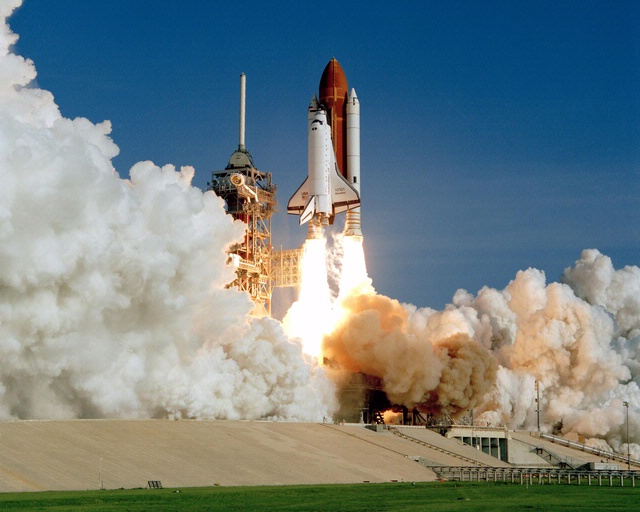
\includegraphics[scale=0.35]{gambar/roketluarangkasa.jpg}

%   % Ubah dengan keterangan gambar yang diinginkan
%   \caption{Peluncuran roket luar angkasa \emph{Discovery} \citep{roketluarangkasa}.}
%   \label{fig:roketluarangkasa}
% \end{figure}

% Roket luar angkasa merupakan \lipsum[1]

% \emph{Discovery}, Gambar \ref{fig:roketluarangkasa}, merupakan \lipsum[2]

\section{Deep Learning}
\label{sec:deeplearning}

Deep Learning sejatinya bagian machine learning yang dimana algoritma nya terinspirasi dari cara kerja jaringan neuron seperti halnya jaringan neuron pada otak manusia. Pada deep learning, syaraf atau neuron merupakan perwakilan dari satu fungsi yang menyimpan suatu nilai atau value yang dimana neuron - neuron ini berada dalam layer - layer yang dimana antar layer memiliki hubungan tertentu. Deep Learning digunakan karena kemampuanya untuk menemukan relasi yang tidak ditemukan antara input dan output. [5]

% \emph{Discovery}, Gambar \ref{fig:roketluarangkasa}, merupakan \lipsum[2]

\section{Convolutional Neural Network}
\label{sec:convolutionalneuralnetwork}

Convolutional Neural Network adalah metode deep learning yang didesain untuk rekognisi pada data dua dimensi yang dimana umumnya berupa gambar visual (tetapi tidak harus berupa gambar) dan untuk klasifikasi. Deep Learning dapat mengatasi masalah dimana terdapat terlalu banyak parameter.  Layer yang biasanya ada di dalam CNN yaitu input layer, convolutional layer, activation layer, dan fully connected layer.
Convolutional layer dan pooling layer merupakan bagian utama pada CNN. Layer - layer tersebut dapat menemukan karakteristik dari objek. Convolutional layer memiliki kapabilitas untuk menemukan dan meningkatkan fitur/karakteristik objek sedangkan pooling layer mampu menyaring fitur fitur yang ditemukan dengan menghapus layer yang tidak diperlukan atau meng-compress fitur. Activation layer memanfaatkan aktivasi non linear untuk meningkatkan expression ability dari model neural network. Fully Connected layer berfungsi untuk menggabungkan fitur - fitur objek dengan nilai output fitur. [6]

% \subsection{Hukum Newton}
% \label{subsec:hukumnewton}

% Newton \citep{newton1687} pernah merumuskan bahwa \lipsum[1]
% Kemudian menjadi persamaan seperti pada persamaan \ref{eq:hukumpertamanewton}.

% % Contoh pembuatan persamaan
% \begin{equation}
%   \label{eq:hukumpertamanewton}
%   \sum \mathbf{F} = 0\; \Leftrightarrow\; \frac{\mathrm{d} \mathbf{v} }{\mathrm{d}t} = 0.
% \end{equation}

% \subsection{Anti Gravitasi}
% \label{subsec:antigravitasi}

% Anti gravitasi merupakan \lipsum[1]


\section{Visi Komputer}
\label{sec:visikomputer}

Convolutional Neural Network adalah metode deep learning yang didesain untuk rekognisi pada data dua dimensi yang dimana umumnya berupa gambar visual (tetapi tidak harus berupa gambar) dan untuk klasifikasi. Deep Learning dapat mengatasi masalah dimana terdapat terlalu banyak parameter.  Layer yang biasanya ada di dalam CNN yaitu input layer, convolutional layer, activation layer, dan fully connected layer.
Convolutional layer dan pooling layer merupakan bagian utama pada CNN. Layer - layer tersebut dapat menemukan karakteristik dari objek. Convolutional layer memiliki kapabilitas untuk menemukan dan meningkatkan fitur/karakteristik objek sedangkan pooling layer mampu menyaring fitur fitur yang ditemukan dengan menghapus layer yang tidak diperlukan atau meng-compress fitur. Activation layer memanfaatkan aktivasi non linear untuk meningkatkan expression ability dari model neural network. Fully Connected layer berfungsi untuk menggabungkan fitur - fitur objek dengan nilai output fitur. [6]

  \cleardoublepage

  % Bab 3 desain dan implementasi
  \chapter{DESAIN DAN IMPLEMENTASI}
\label{chap:desainimplementasi}

% Ubah bagian-bagian berikut dengan isi dari desain dan implementasi
Judul penelitian "Deteksi Helm Keselamatan Kerja Menggunakan CNN" mengikuti metode atau desain sistem berikut serta impelementasinya.
Pada gambar berikut menunjukkan bagan umum metodologi sistem dari penelitian.

\begin{figure}[ht]
  \centering
  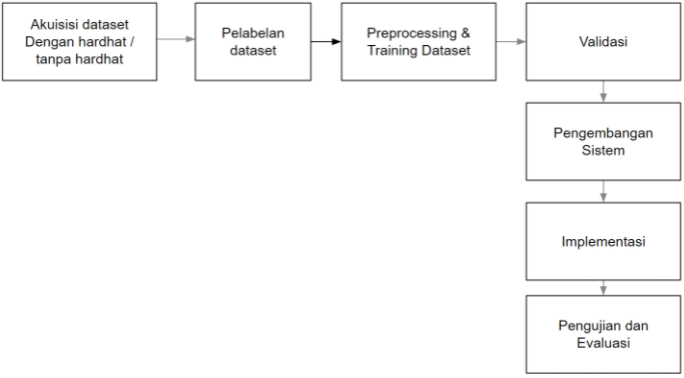
\includegraphics{gambar/blockdiagram-helmetdetection.png}
  \caption{Block Diagram Helmet Detection}
  \label{fig:helmetdetectiondiagram}
\end{figure}

\section{Desain Sistem}
\par Judul ini merupakan penelitian di bidang \emph{computer vision} 


\section{Deskripsi Sistem}
\label{sec:deskripsisistem}

Sistem akan dibuat dengan \lipsum[1-2]

\section{Implementasi Alat
\label{sec:implementasi alat}}

Alat diimplementasikan dengan \lipsum[1]

% Contoh pembuatan potongan kode
\begin{lstlisting}[
  language=C++,
  caption={Program halo dunia.},
  label={lst:halodunia}
]
#include <iostream>

int main() {
    std::cout << "Halo Dunia!";
    return 0;
}
\end{lstlisting}

\lipsum[2-3]

% Contoh input potongan kode dari file
\lstinputlisting[
  language=Python,
  caption={Program perhitungan bilangan prima.},
  label={lst:bilanganprima}
]{program/bilangan-prima.py}

\lipsum[4]

  \cleardoublepage
  
  % Bab 4 pengujian dan analisis
  \chapter{PENGUJIAN DAN ANALISIS}
\label{chap:pengujiananalisis}

% Ubah bagian-bagian berikut dengan isi dari pengujian dan analisis

Pada penelitian ini dipaparkan \lipsum[1][1-5]

\section{Skenario Pengujian}
\label{sec:skenariopengujian}

Pengujian dilakukan dengan \lipsum[1-2]

\section{Evaluasi Pengujian}
\label{sec:analisispengujian}

Dari pengujian yang \lipsum[1]

% Contoh pembuatan tabel
\begin{longtable}{|c|c|c|}
  \caption{Hasil Pengukuran Energi dan Kecepatan}
  \label{tb:EnergiKecepatan}\\
  \hline
  \rowcolor[HTML]{C0C0C0}
  \textbf{Energi} & \textbf{Jarak Tempuh} & \textbf{Kecepatan} \\
  \hline
  10 J & 1000 M & 200 M/s \\
  20 J & 2000 M & 400 M/s \\
  30 J & 4000 M & 800 M/s \\
  40 J & 8000 M & 1600 M/s \\
  \hline
\end{longtable}

\lipsum[2-4]

  \cleardoublepage

  % Bab 5 penutup
  \chapter{PENUTUP}
\label{chap:penutup}

% Ubah bagian-bagian berikut dengan isi dari penutup

\section{Kesimpulan}
\label{sec:kesimpulan}

Berdasarkan hasil pengujian yang \lipsum[1][1-3] sebagai berikut:

\begin{enumerate}[nolistsep]

  \item Pembuatan \lipsum[2][1-3]

  \item \lipsum[2][4-6]

  \item \lipsum[2][7-10]

\end{enumerate}

\section{Saran}
\label{chap:saran}

Untuk pengembangan lebih lanjut pada \lipsum[1][1-3] antara lain:

\begin{enumerate}[nolistsep]

  \item Memperbaiki \lipsum[2][1-3]

  \item \lipsum[2][4-6]

  \item \lipsum[2][7-10]

\end{enumerate}

  \cleardoublepage

  % Daftar pustaka
  \renewcommand\bibname{DAFTAR PUSTAKA}
  \addcontentsline{toc}{chapter}{\bibname}
  \bibliographystyle{unsrtnat}
  \bibliography{pustaka/pustaka.bib}
  \cleardoublepage

  % Biografi penulis
  \begin{center}
  \Large
  \textbf{BIOGRAFI PENULIS}
\end{center}

\addcontentsline{toc}{chapter}{BIOGRAFI PENULIS}

\vspace{2ex}

\begin{wrapfigure}{L}{0.3\textwidth}
  \centering
  \vspace{-3ex}
  % Ubah file gambar berikut dengan file foto dari mahasiswa
  
\includegraphics[width=0.3\textwidth]{gambar/elon.jpg}
  \vspace{-4ex}
\end{wrapfigure}

% Ubah kalimat berikut dengan biografi dari mahasiswa
Elon Reeve Musk, lahir pada \lipsum[1]

\lipsum[2]

  \cleardoublepage

\end{document}
